\documentclass{standalone}
\usepackage{hsbcommon}
\makeatletter\AtBeginDocument{\@buildstepset{0,1,2,3,4,5,6,7,8}}\makeatother
\begin{document}
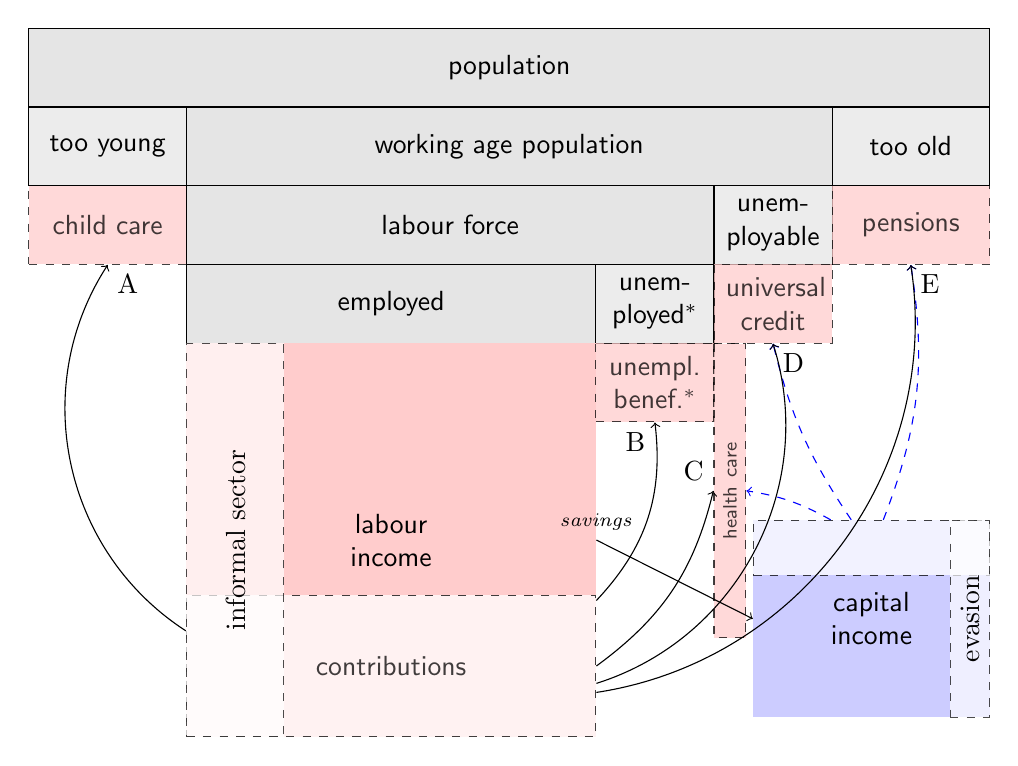
\begin{tikzpicture}
    % -------------------------------------------------------------------
    % STEP 1 of 2: only the "employed" column is resized.
    %
    % Original widths (too young=2, employed=3, unemployed=1.5,
    % not employable=1.5, too old=2; total=10) were all within ~10-15%
    % of real UK Labour Force Survey shares (~18%, ~47%, ~2.5%, ~13%,
    % ~19%) EXCEPT "employed", which was far too small.
    %
    % Calibration: using the three columns treated as already-accurate
    % (too young=2, not employable=1.5, too old=2; sum=5.5cm <-> ~50%
    % of population in reality) gives a scale of ~0.11 cm per 1% of
    % population. Employed's real share (~47%) then implies:
    %     employed width = 47 * 0.11 =~ 5.2cm  (was 3cm, so +2.2cm)
    %
    % Everything to the right of "employed" (unemployed, not employable,
    % too old, and their annotation boxes below) is shifted right by
    % the same +2.2cm. The "unemployed" box itself is NOT resized here
    % -- that is step 2.
    % -------------------------------------------------------------------
    \tikzset{
        myboxed/.style={
                draw,
                minimum height=1cm,
                anchor=west,
                fill=gray!20,
                align=center,
                font=\sffamily
            },
        mywages/.style={
                % draw,
                minimum height=1cm,
                anchor=west,
                fill=red!20,
                align=center,
                font=\sffamily       
        },        
        mygains/.style={
                % draw,
                minimum height=1cm,
                anchor=west,
                fill=blue!20,
                align=center,
                font=\sffamily       
        },
        mytransfer/.style={
                minimum height=1cm,
                anchor=west,
                fill=white,
                opacity=0.75,
                draw, 
                dashed,
                align=center,
                font=\sffamily       
        }, 
        mybenefit/.style={
                minimum height=1cm,
                anchor=west,
                fill=red!20,
                opacity=0.75,
                draw,dashed,  
                align=center,
                font=\sffamily       
        },
        unboxed/.style={
                minimum height=1cm,
                fill=gray!15,
                draw,
                anchor=west,
                font=\sffamily
            }
        }
    \node[myboxed,minimum width=12.2cm] at (0,0) {population};
    \node[myboxed,minimum width=8.2cm] at (2,-1) {working age population};
        \node[unboxed,minimum width=2cm] at (0,-1) {too young};
        \node[unboxed,minimum width=2cm] at (10.2,-1) {too old};
    \node[myboxed,minimum width=6.7cm] at (2,-2) {labour force};
        \node[unboxed,minimum width=1.5cm,
        text width=1.2cm,align=center] at (8.7,-2) {un\-em\-ploy\-able};
    \node[myboxed,minimum width=5.2cm] at (2,-3) {employed};
        \node[unboxed,minimum width=1.5cm,text width=1.2cm,align=center] at (7.2,-3) {un\-em\-ployed$^*$};

    \ifsteponly{1}{2,3,4}{
        \node[anchor=west, minimum width=5cm] at (2,-4) {long-term \& short-term};
        \node[anchor=west, minimum width=5cm] at (2,-4.5) {skilled \& non-skilled};
    }

    \ifstep{2}{
       \node[mywages,minimum width=5.2cm,text width=2cm, minimum height=5cm] (wages) at (2,-6) {labour income};
    }

    \ifstep{3}{
        \node[mybenefit,minimum width=2cm,text width=1.5cm] (childcare) at (0,-2) {child care};
    }
    \ifstep{3}{
        \node[mybenefit,minimum width=1.5cm,text width=1.2cm] (benefits) at (7.2,-4) {unempl. benef.$^*$};
    }
     \ifstep{3}{
        \node[mybenefit,minimum width=1.5cm,text width=1.2cm] (credit) at (8.7,-3) {universal credit};
    }
    \ifstep{3}{
        \node[mybenefit,minimum height=1ex, anchor=north east,text width=3.5cm,rotate=90] (healthcare) at (8.7,-3.5) {\scriptsize health care};
    }
    \ifstep{3}{
        \node[mybenefit,minimum width=2cm,text width=1.5cm] (pensions) at (10.2,-2) {pensions};
    }

    \ifstep{5}{%% capital gains
       \node[mygains,minimum width=3cm,text width=2cm, minimum height=2.5cm] (gains) at (9.2,-7) {capital income};
    }

    \ifstep{6}{
        \node[mytransfer,minimum width=3cm,minimum height=0.7cm] (transfer2) at(9.2,-6.1) {} ;
        \draw[dashed,blue,->,bend right=15] (transfer2) to (pensions.south);
        \draw[dashed,blue,->,bend left=10] (transfer2) to (credit.south);
        \draw[dashed,blue,->,bend right=10] (transfer2) to (healthcare.south);
        % \draw[dashed,blue,->,bend left=10] (transfer2) to (benefits.south);
        % \draw[dashed,blue,->,bend left=10] (transfer2.west) to (childcare.south);
    }

    \ifstep{4}{%% transfers
        \node[mytransfer,minimum width=5.2cm,minimum height=1.8cm] (transfer) at(2,-7.6) {contributions} ;
        \draw[->,bend left=45] (transfer) to (childcare.south) node[below right] {A};
        \draw[->,bend right=25] (transfer) to (benefits.south) node[below left] {B};
        \draw[->,bend right=20] (transfer.east) to (healthcare.north) node[above left] {C} ;
        \draw[->,bend right=45] (transfer) to (credit.south) node[below right] {D};
        \draw[->,bend right=45] (transfer) to (pensions.south) node[below right] {E} ;
    }

    \ifstep{6}{%% transfers hohe Löhne zu niedrigen
        \draw[->] (wages.east) node[above]{\scriptsize \textit{savings}} to  (gains.west) ;
    }

    \ifstep{7}{%% schattenwirtschaft Kapital
       \node[mygains,minimum width=0.5cm, minimum height=2.5cm,opacity=0.7,anchor=west,draw,fill=white,dashed] (informalgains) at (11.7,-7) {};
       % \node[mywages,minimum width=1cm,text width=1cm,minimum height=5cm,draw,dashed,fill=white,opacity=0.7,anchor=west] (shadow) at (2,-6) {};
       \node[rotate=90,anchor=north,minimum height=0.5cm] (shadowcap) at (11.7,-7) {evasion};
    }
    
    \ifstep{8}{
       \node[mywages,minimum width=1cm,text width=1cm,minimum height=5cm,draw,dashed,fill=white,opacity=0.7,anchor=west] (shadow) at (2,-6) {};
       \node[rotate=90,anchor=north,minimum height=1.25cm] (shadow) at (2,-6) {informal sector};
    }
    
    
\end{tikzpicture}
\end{document}